\documentclass[12pt,a4paper]{article}
\usepackage[utf8]{inputenc}
\usepackage{graphicx}


\renewcommand*\familydefault{\sfdefault} 
\usepackage{ragged2e}
\usepackage{multicol} % Paquete para dos columnas

\title{SRS: Sistema de Venta y distribución de textiles para el sector industrial con enfoque a vestidos de gala.}
\author{
	\begin{tabular}{c}
		Armenta Telles Jesús Manuel, Contreras Rangel Martin, \\
		Diaz Escalante José Ángel, 
		Higuera Sánchez Dulce Mariela, \\
		Reyes Contreras Ramsés, 
		Rodríguez Cacho Ximena Charleene \\
	\end{tabular}
}
\date{\today}



\begin{document}
	\maketitle
	
	\begin{multicols}{2} % Inicia entorno de dos columnas
		\section{Introducción}
		El presente documento tiene por objeto desarrollar una aplicación web que gestione la administación de recursos (materia prima) y maneje una correcta logistica con sus materiales, así como distribuirlos a sus tres sucursales y tener un control de ventas sobre el mismo, para que de esta manera se cuenta con una organización óptima y un manejo eficiente de sus productos, evitanto así tener pérdidas monetarias.
		
		\section{Objetivo}
		Optimizar las operaciones comerciales de la empresa a traves de una app web, reduciendo pérdidas en recursos y ofreciendo una experiencia intuitiva para los clientes, facilitando la búsqueda, selección y compra de productos desde un dispositivo movil. 
		
		\section{Descripción del proyecto}
		Es una aplicación enfocada en administrar las ventas
		producidas, le permitirá a la empresa gestionar sus diversos catálogos (de clientes,
		de proveedores) así como sus inventarios (de materia y de los lotes de vestidos),
		para así lograr venderlos a los clientes, a través de una interfaz intuitiva. \linebreak  
		
		Este proyecto soluciona los problemas de la empresa, con la finalidad de evitar pérdidas
		monetarias. El administrador será capaz de actualizar los catálogos e inventarios, así como
		agregar nuevos elementos, podrá modificar, eliminar y consultar las existencias del
		momento. \linebreak  
		
		Los potenciales clientes podrán solicitar en la aplicación web el tipo de vestido
		deseado por lote, y las cantidades que componen el lote vendrá indicado en la
		descripción, contarán con su perfil individual, con el cual podrán visualizar en la
		interfaz web los productos, agregarlos a un “carrito de compras”, y decidir si
		modificara su solicitud, cancelar la solicitud o simplemente consultar sus facturas
		realizadas, además de tener acceso a modificar su perfil de usuario.
		
		\section{Carácteristicas del sistema}
		De forma general, este se enfocará en gestione la administración de recursos, y que coordine eficientemente la logística de distribución hacia las tres sucursales de la empresa. Además, el sistema controlará las ventas, ofreciendo una aplicación intuitiva para usuarios y administradores, permitiendo la gestión de catálogos de productos, clientes y proveedores, así como la realización de pedidos, Y la gestión del carrito de compras.
		
		\section{Funcionalidades generales}
		El sistema contará con las siguientes carácteristicas fundamentales para su correcto funcionamiento:
		
		\begin{itemize}
			\item     Registro de materia prima y otros recursos.
			\item Gestión de inventario de materiales y productos.
			\item Coordinación logística para la distribución a las sucursales.
			\item Control de ventas, incluyendo catálogos de productos, clientes y proveedores.
			\item Plataforma intuitiva para usuarios y administradores.
			\item Realización de pedidos y gestión de carrito de compras.
			\item Registros de compras.
			\item Actualización de catálogos e inventarios por parte de los administradores.
			\item Funciones de modificación, eliminación y consulta de existencias.
			\item Organización eficiente de productos y recursos de la empresa.
		\end{itemize}
		
		\section{Requerimientos de la aplicación}
		La aplicación tiene por nombre de software: Galatex, sus requerimientos son:
		
		\begin{itemize}
			\item Inventario: 
			\subitem  Se manejará un inventario donde se
			tenga catalogado cada material y
			producto con el que contamos, para así
			facilitar el control y nuestro manejo de
			materiales.
			
			\item Catálogo de productos:
			\subitem Se tendrá un inventario donde se
			muestren todos productos disponibles
			en el momento (los lotes de vestido), y
			en caso de estar agotado igual se
			mostrará en pantalla.
			
			\item Catálogo de proveedores
			\subitem Se tendrá registrado cada proveedor de
			material, guardando información como
			el nombre de la empresa, ubicación, su
			código de referencia fiscal y el material
			que nos surten.
			
			\item Catálogo de clientes
			\subitem Así como se tendrá un catálogo de
			proveedores, a la vez se tendrá uno
			para los clientes, para que, a la vez, se
			organicen los pedidos de forma que
			sepamos que cliente realizo el pedido y
			de qué forma podemos contactarlo
			
			\item Registro e inicio de sesión para cliente
			\subitem Para que el cliente pueda ingresar a
			nuestra página web y realizar un
			pedido, tendrá que primero registrarse
			en nuestro sitio web e ingresar la
			información que se le pide (Correo,
			nombres, apellidos, contraseña,
			número telefónico, y su RFC), ya que
			esta información se haya ingresado, el
			perfil se creará y el cliente podrá iniciar
			sesión cuando desee.
			
			\item Modificación y eliminación de
			información del cliente
			\subitem En la página, el cliente podrá ser capaz
			de alterar su información, como su
			nombre, contraseña, correo, etc. Así
			como también eliminar su cuenta si ya
			no requiere de los servicios que le
			ofrecemos, esto solamente podra pasar
			si el usuario no tiene una compra
			registrada en su cuenta, si es asi,
			tendrá que hablar con el administrador
			con anterioridad.
			
			\item Alta y baja de proveedores
			\subitem Un administrador será capaz de dar el
			alta, así como baja de sus proveedores
			que ya no estén activos con la empresa.
			
			\item Carrito de compras
			\subitem El cliente podrá seleccionar sus
			productos que desea comprar en una
			lista previa, con la opción de poder
			borrar algún producto, o proceder al
			pago.
			
			\item Recuperación de Contraseña
			\subitem Si al cliente se le llegara a olvidar su
			contraseña, tendría la opción de
			recuperarla por medio de su correo.
			
			
		\end{itemize}github
		
	\end{multicols} 
	
	\section{Diagramas del proyecto}
	
	\subsection{Diagrama entidad relacion}
	\begin{figure}[h]
		\centering
		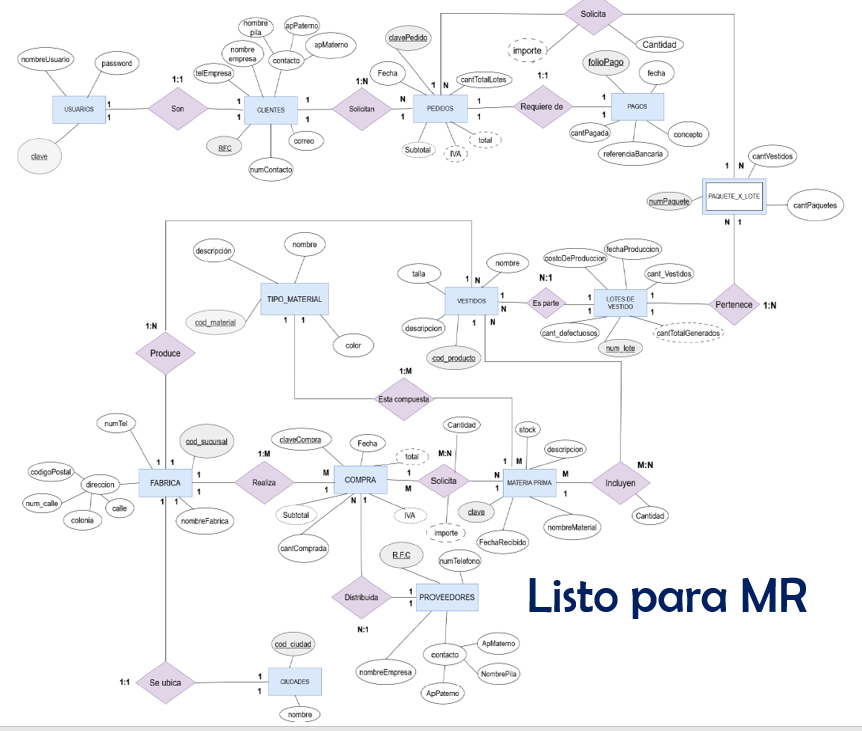
\includegraphics[width=0.5\textwidth]{der.png}
		\caption{Diagrama Entidad relacion.}
		\label{fig: 1. Diagrama Entidad relacion.}
	\end{figure}
	
	
	\subsection{Modelo relacional}
	\begin{figure}[h]
		\centering
		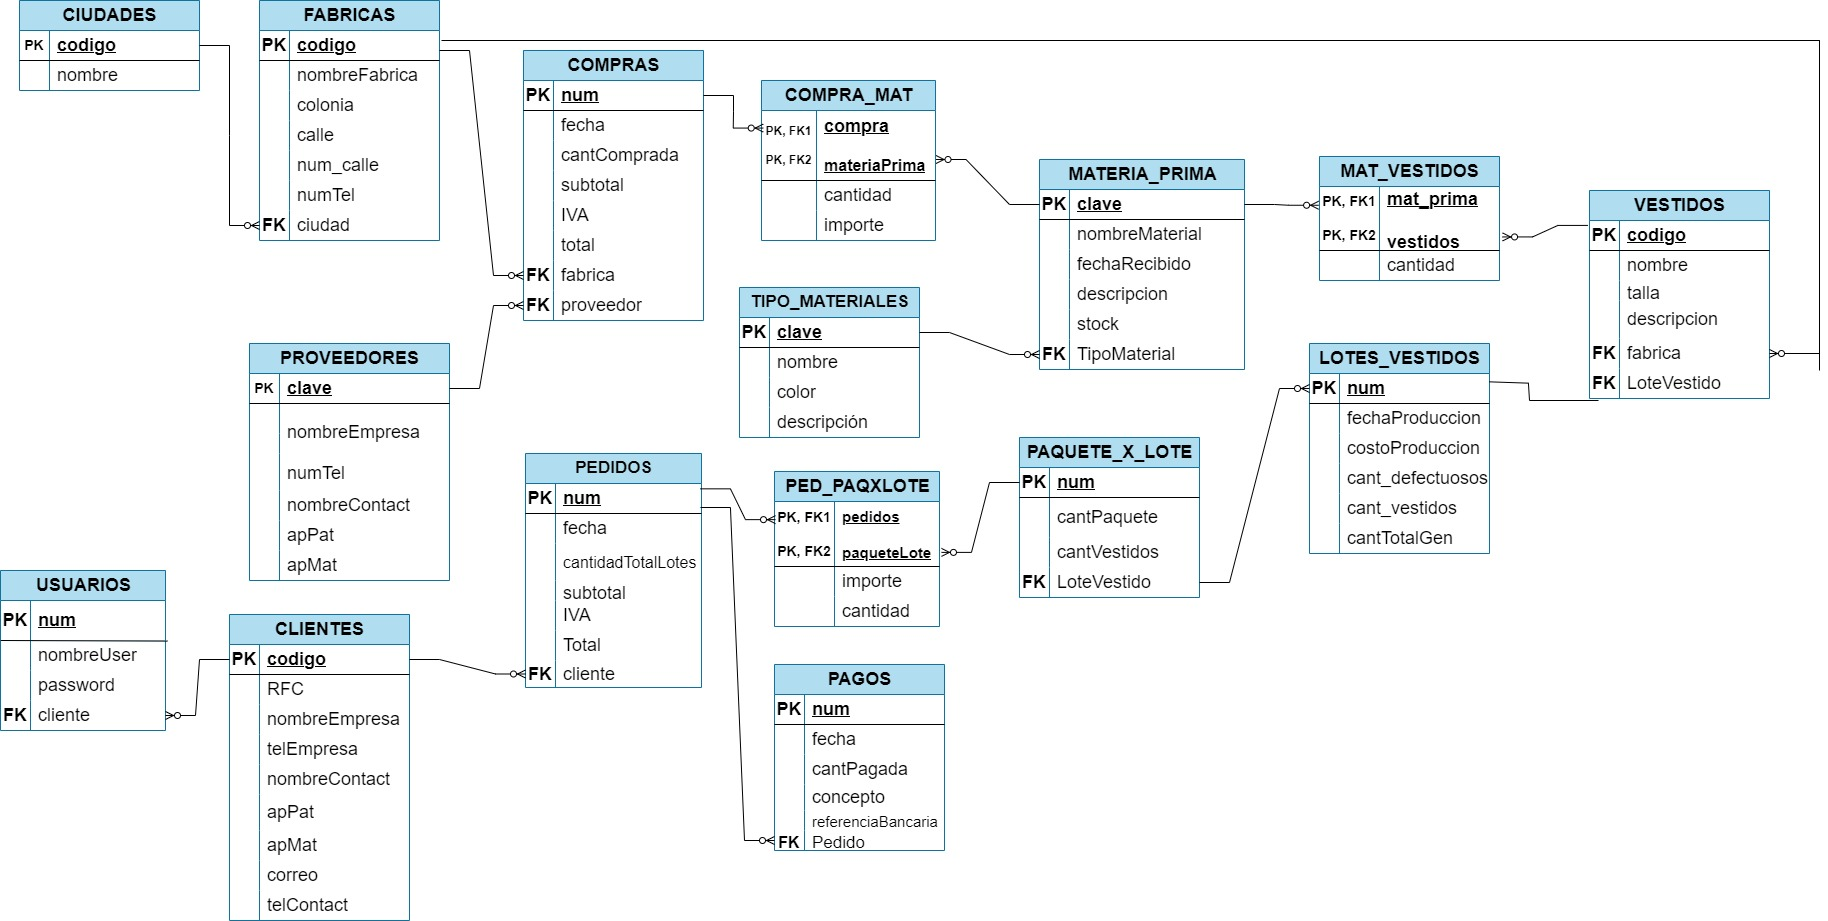
\includegraphics[width=0.5\textwidth]{mrgalatex.jpeg}
		\caption{Diagrama Modelo relacional.}
		\label{fig: 2. Modelo relacional.}
	\end{figure}
	\newpage
	\subsection{Casos de uso}
	\begin{figure}[h]
		\centering
		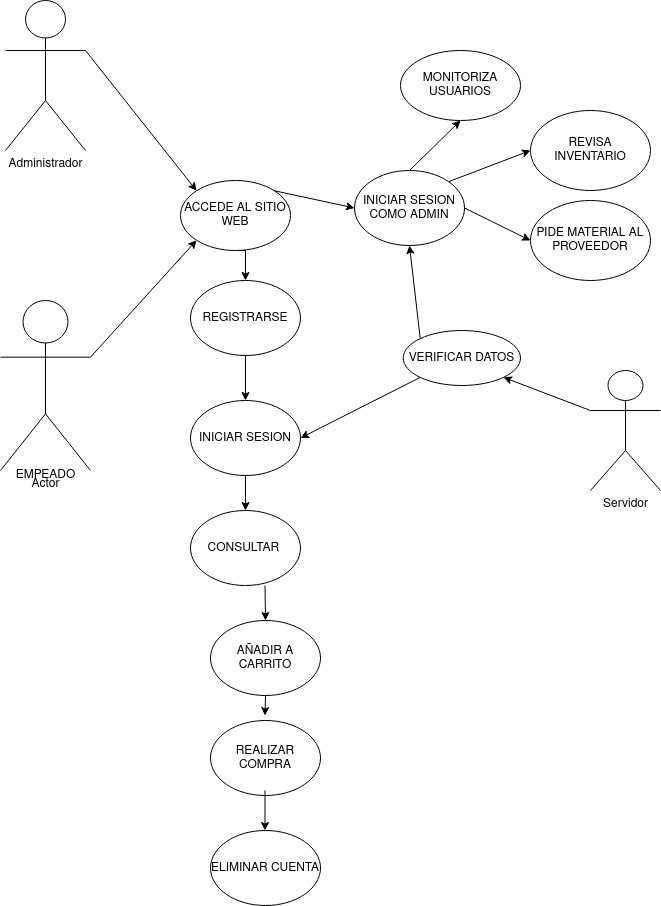
\includegraphics[width=0.5\textwidth]{casosUso.jpg}
		\caption{Diagrama Casos de uso.}
		\label{fig: 1. Diagrama casos de uso}
	\end{figure}
	
	\newpage % Inserta un salto de página aquí
	
	\section{Asignación y validación}
	El equipo involucrado se compromete a desarrollar lo descrito en el presente documento, cumpliendo con cada uno de las requerimientos descritos para que la aplicación sea un producto de calidad y que sea funcional.\linebreak  
	El docente al firmar acepta lo descrito en el presente documento para el posterior desarrollo del proyecto.\linebreak\linebreak   
	
	Firma de connformidad: \underline{\hspace{4cm}}\linebreak\linebreak 
	Firma equipo desarrollador: \underline{\hspace{4cm}}\linebreak 
	
\end{document}
